\documentclass{standalone}
\usepackage{tikz}
\usepackage{ctex,siunitx}
\setCJKmainfont{Noto Serif CJK SC}
\usepackage{tkz-euclide}
\usepackage{amsmath}
\usetikzlibrary{patterns, calc}
\usetikzlibrary {decorations.pathmorphing, decorations.pathreplacing, decorations.shapes,}

\begin{document}
\small
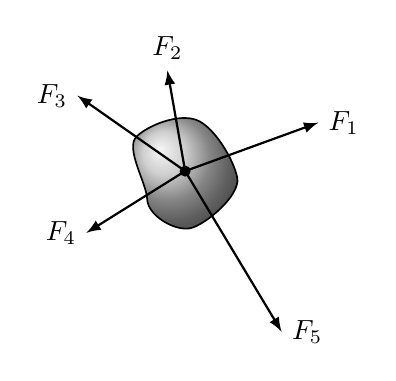
\begin{tikzpicture}[>=latex,scale=1]
  % \useasboundingbox(-0.25,-0.25)rectangle(4,3);
  \draw[semithick,ball color=lightgray](-0.482,-0.358)..controls(-0.473,-0.570)and(-0.123,-0.768)..
  ( 0.068,-0.725)..controls( 0.258,-0.682)and( 0.704,-0.309)..
  ( 0.662,-0.085)..controls( 0.620, 0.139)and( 0.372, 0.561)..
  ( 0.147, 0.648)..controls(-0.079, 0.736)and(-0.461, 0.587)..
  (-0.615, 0.441)..controls(-0.770, 0.294)and(-0.491,-0.146)..cycle;
  \fill(0,0)circle(2pt);
  \draw[->,thick](0,0)--(20:1.8)node[right]{$F_1$};
  \draw[->,thick](0,0)--(100:1.3)node[above]{$F_2$};
  \draw[->,thick](0,0)--(145:1.67)node[left]{$F_3$};
  \draw[->,thick](0,0)--(212:1.48)node[left]{$F_4$};
  \draw[->,thick](0,0)--(-59:2.38)node[right]{$F_5$};
\end{tikzpicture}
\end{document}